The developed variant of the k-Means algorithm was tested by implementing the classical k-Means algorithm (Lloyd's algorithm), Elkan's algorithm, and the Ptolemy-based extension in Python. The code is available on GitHub~\cite{Averitchev2024kMeansPtolemy}. To provide a fair comparison, a variable was included to count the number of distance calculations for each algorithm. This metric was chosen because distance calculations account for the majority of computing time in k-Means algorithms, offering a clear measure of efficiency regardless of implementation optimizations.

Additionally, two intermediate variants were implemented to assess the separate effects of the lower and upper bounds: one uses Elkan's lower bound with Ptolemy's upper bound, and the other uses Ptolemy's lower bound with Elkan's upper bound. 

\subsection{Datasets}

A variety of datasets were used to compare the performance of the algorithms. The datasets are summarized in Table~\ref{tab:datasets}. 
\begin{table}[htbp]
\centering
\caption{Datasets Used in the Experiments}
\label{tab:datasets}
\begin{tabular}{lll}
\hline
\textbf{Dataset} & \textbf{Cardinality} & \textbf{Dimensionality} \\
\hline
\multicolumn{3}{l}{\textit{Fixed-Structure Datasets}} \\
Iris & 150 & 4 \\
Wine & 178 & 13 \\
\hline
\multicolumn{3}{l}{\textit{Variable-Dimension Datasets}} \\
Gaussian Low Dimension & 10,000 & 10 \\
Gaussian Medium Dimension & 10,000 & 100 \\
Gaussian High Dimension & 10,000 & 300 \\
Random Low Dimension & 5,000 & 10 \\
Random Medium Dimension & 5,000 & 100 \\
Random High Dimension & 5,000 & 300 \\
\hline
\end{tabular}
\end{table}

The fixed-structure datasets include the Iris and Wine datasets \cite{pedregosa2011scikit}, which have fixed dimensions and cardinalities and represent different clustering structures. The variable-dimension datasets include Gaussian and Uniform Random datasets, which offer flexibility in terms of dimensionality and cardinality, making them ideal for testing the algorithms under various conditions.

\subsection{Experiments}

The experiments were designed to evaluate the algorithms based on the number of distance calculations, which dominate the computing time in k-Means algorithms. This metric ensures comparability across different implementations and hardware setups. Each algorithm was executed three times on each dataset, with the parameters $k = 3$, $k = 20$, and $k = 100$.

The results for the Iris and Wine datasets are visualized in Fig. \ref{fig:wine+iris}, while Fig. \ref{fig:gauss_univariate} illustrates the performance on the Random and Gaussian dataset variations. These figures present the speedup relative to Elkan's algorithm, showcasing any improvements introduced by the proposed extension.


\begin{figure}
  \centering
  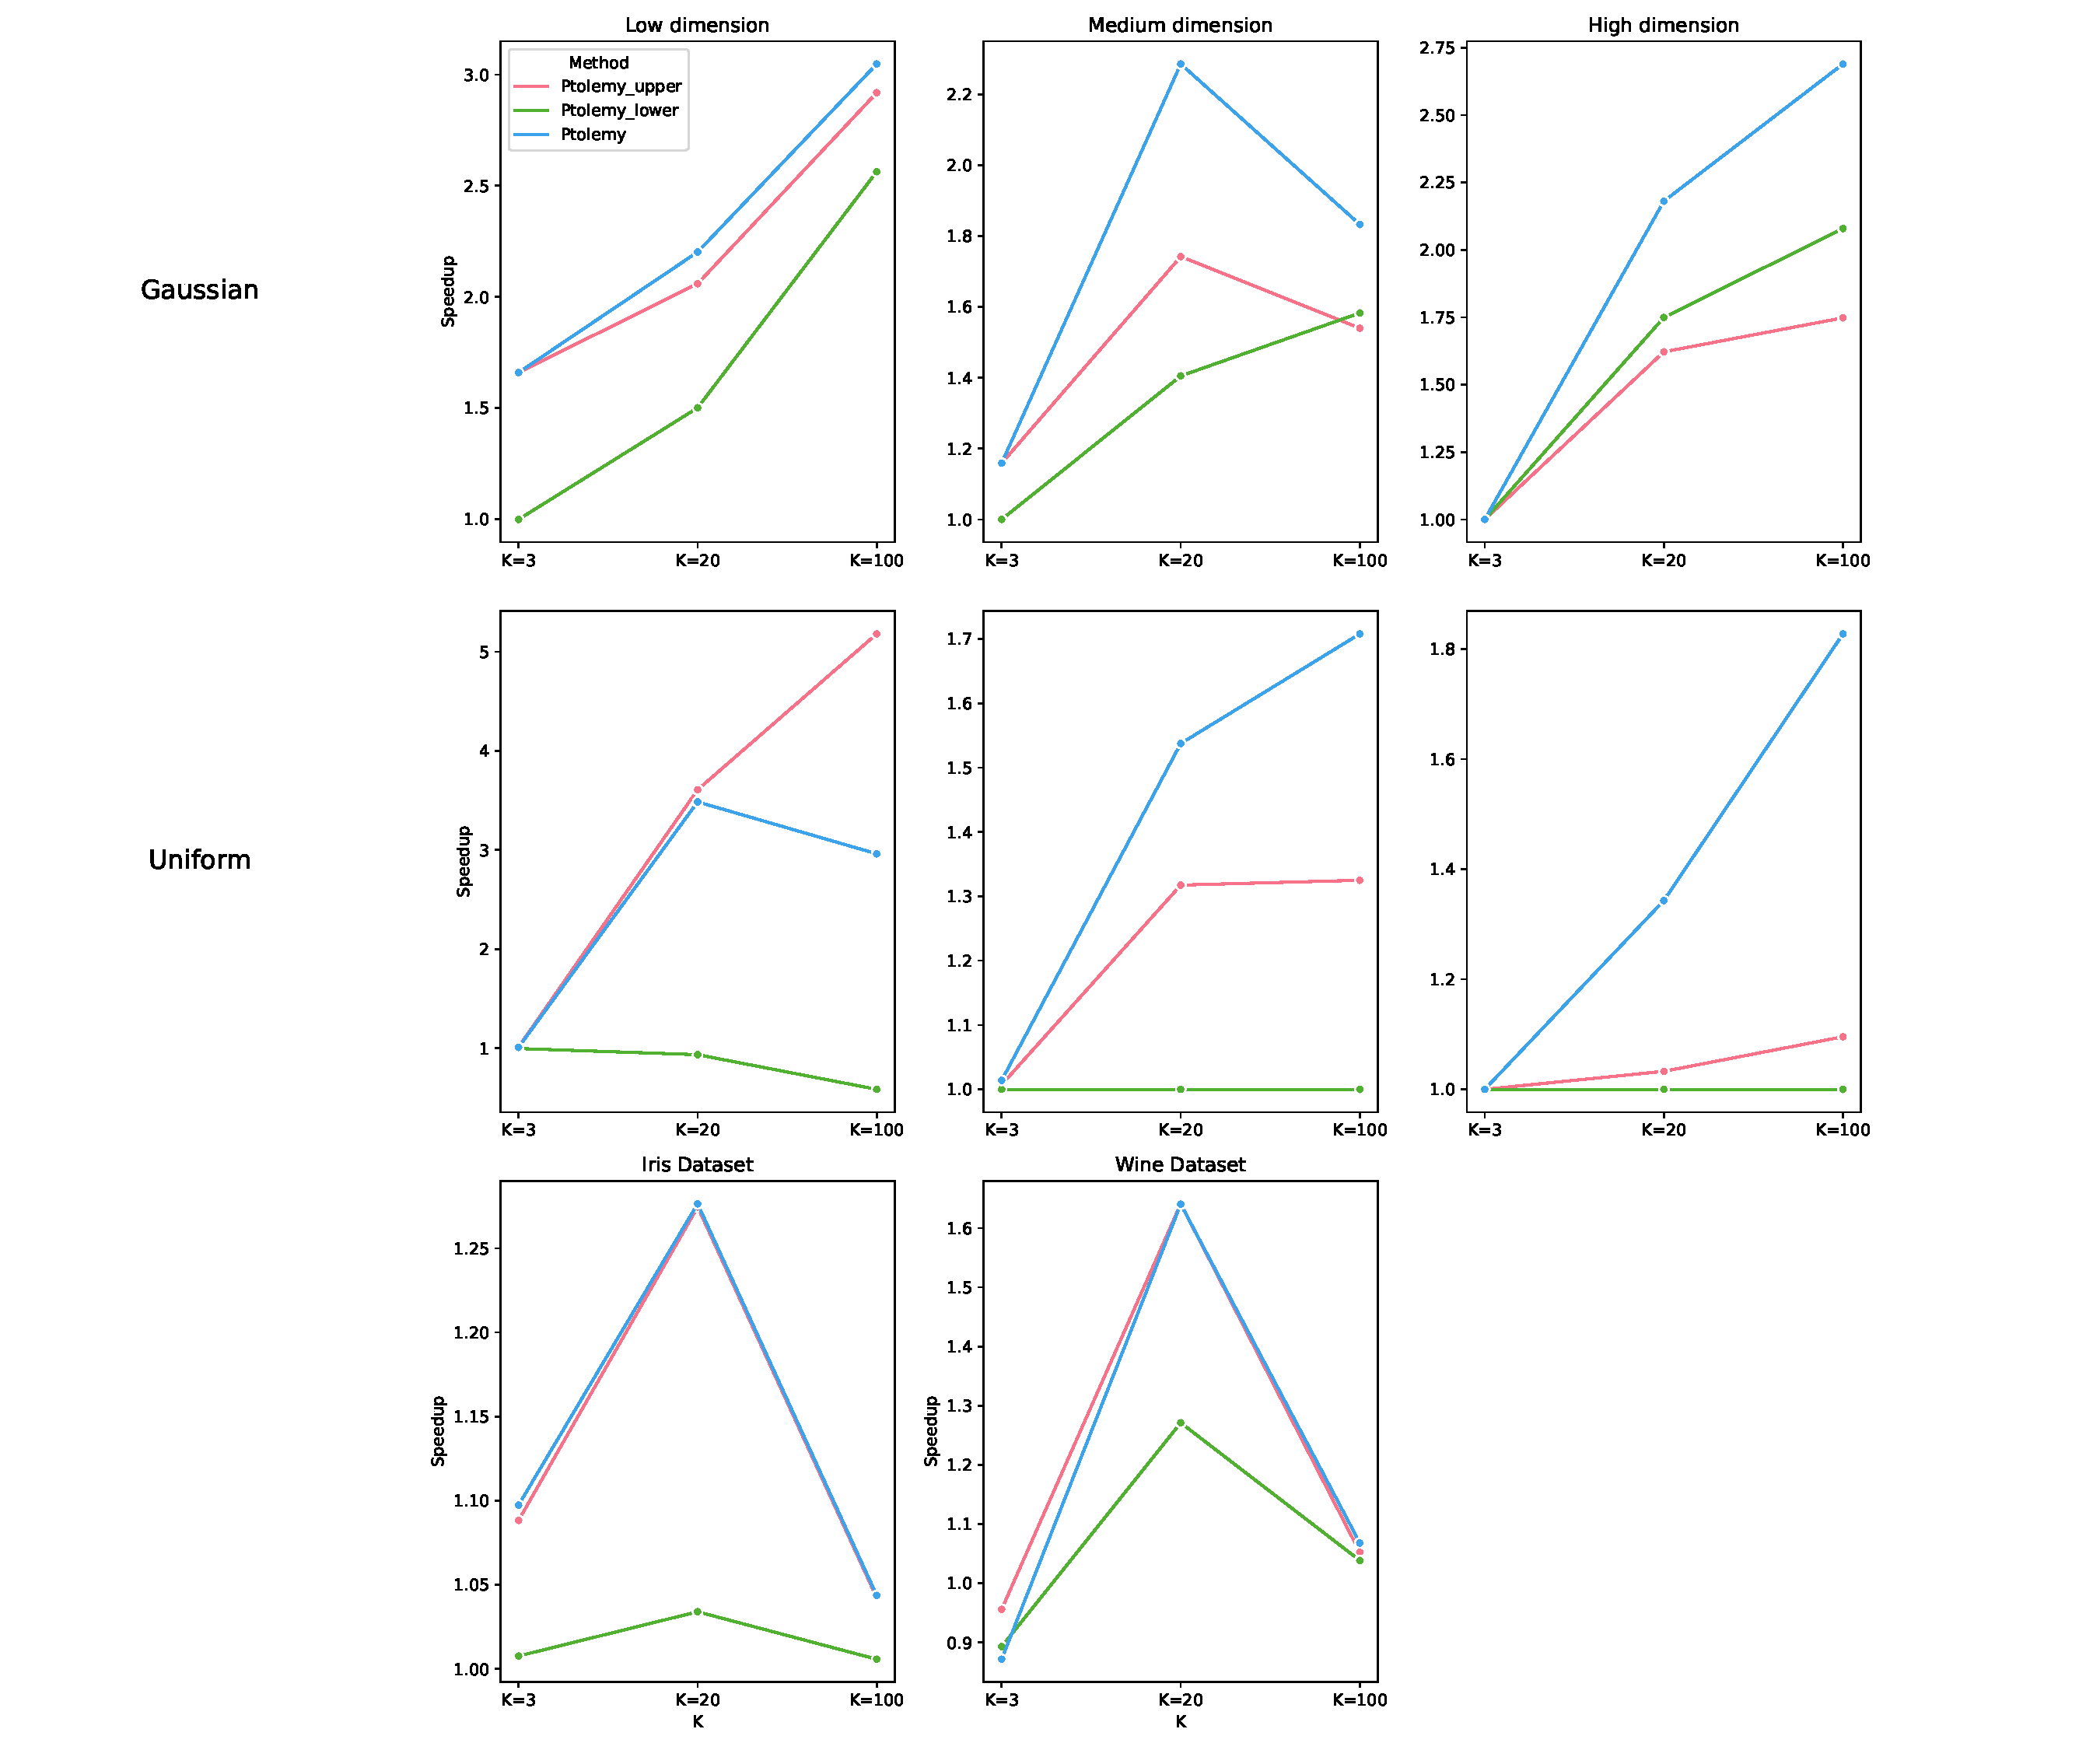
\includegraphics[width=\textwidth]{fig/combined_plot.pdf}
  \caption{}
  \label{fig:combined}
\end{figure}


\subsection{Analysis of the Results}

The experimental results, presented in the figures, provide critical insights into the performance of the k-Means algorithm variants. The primary focus of this analysis is on the full Ptolemaic algorithm and its comparison with Elkan’s algorithm. The results highlight several scenarios in which the full Ptolemaic algorithm achieves substantial improvements over Elkan’s approach, particularly in reducing the number of distance evaluations.

\textbf{Influence of the Number of Clusters}

The full Ptolemaic algorithm consistently demonstrates notable improvements over Elkan’s algorithm as the number of clusters ($k$) increases. For instance, in the Gaussian low-dimensional dataset, the Ptolemaic algorithm achieves speedups of over 2-fold for $k = 20$ and surpasses 3-fold for $k = 100$, illustrating its ability to significantly reduce distance calculations in more complex clustering tasks. Similar trends are observed in the Random low-dimensional dataset, where the full Ptolemaic algorithm achieves a speedup of more than 3-fold at $k = 20$ and $k = 100$. These results underscore the increasing efficiency of the Ptolemaic algorithm as the clustering complexity grows.

In contrast, for smaller cluster counts, such as $k = 3$, the performance advantage of the full Ptolemaic algorithm is less pronounced but still evident, with speedups of around 1.1 in both the Iris and Wine datasets. This suggests that while Ptolemy’s inequality offers significant improvements for larger $k$ values, it still provides moderate gains for smaller cluster sizes.

The Ptolemaic Upper Bound variant performs comparably to the full Ptolemaic algorithm, especially for larger $k$ values, delivering similar efficiency improvements. However, the Ptolemaic Lower Bound variant tends to underperform in some cases, particularly with smaller cluster counts or in higher-dimensional datasets, where its speedup is sometimes close to or even below that of Elkan’s algorithm.

\textbf{Influence of Dimensionality}

The full Ptolemaic algorithm also performs well across datasets with varying dimensionality. In the Gaussian low-dimensional dataset (10 dimensions), the full Ptolemaic algorithm achieves impressive speedups, particularly at higher cluster counts, with speedups over 3-fold at $k = 100$. As the dimensionality increases, the performance gains of the Ptolemaic algorithm persist, though they become slightly less pronounced. For example, in the Gaussian medium (100 dimensions) and Gaussian high (300 dimensions) datasets, the Ptolemaic algorithm continues to offer significant speedups, but the performance advantage over Elkan’s algorithm decreases slightly.

In higher-dimensional datasets, such as the Random high-dimensional dataset, the full Ptolemaic algorithm remains effective, consistently reducing the number of distance evaluations, particularly for larger $k$ values. However, the Ptolemaic Lower Bound variant often struggles in these higher-dimensional cases, further emphasizing the robustness of the full Ptolemaic approach.

\textbf{Summary of Results}

The full Ptolemaic algorithm demonstrates consistent and significant improvements over Elkan’s algorithm across a variety of datasets, particularly in scenarios with a high number of clusters and low to medium dimensionality. The Ptolemaic Upper Bound variant performs similarly in many cases, offering comparable efficiency gains, whereas the Ptolemaic Lower Bound variant sometimes struggles, particularly in datasets with higher dimensionality or smaller cluster counts. Overall, the full Ptolemaic algorithm proves to be a robust and efficient alternative to traditional k-Means implementations, especially as the complexity of the clustering task increases.